\documentclass[a4paper,11pt,spanish, twoside, leqno]{tfg-uam}

\usepackage[utf8]{inputenc}
\usepackage{amsfonts, amssymb, amsmath, amsthm}
\usepackage{graphicx}
\usepackage{color}

\newtheorem{teor}{Teorema}[chapter]
\newtheorem{lema}[teor]{Lema}
\newtheorem*{teorsin}{Teorema}


\theoremstyle{definition}
\newtheorem{defin}[teor]{Definici\'on}

\title{Teorema de clasificación de superficies}
\author{Rodrigo De Pool}
\tutor{Javier Aramayona}
\curso{2019-2020}


%%%%%METADATOS: rellenar la info solicitada entre llaves
\usepackage{hyperref}
\hypersetup{
	pdfinfo={
            Title={Teorema de clasificaci\'on de superficies }, %Titulo del trabajo; ejemplo: Matematicas y desarrollo
            Author={ Rodrigo De Pool}, %Autor del trabajo; ejemplo: Juan Sanchez
            Director1={javier.aramayona }, %Tutor1: en formato nombre.apellido, tal como aparece en la primera parte, antes de la arroba,  de su direcci�n de correo electr�nico de la UAM; ejemplo: fernando.soria
            Director2={ }, %Tutor2: en formato nombre.apellido, tal como aparece en la primera parte, antes de la arroba,  de su direcci�n de correo electr�nico de la UAM
            Ndirectores={1 }, %Numero total de directores: 1 � 2
            Tipo={TFG}, %no tocar
            Curso={2018-19}, %no tocar
            Palabrasclave={ },% Palabras clave del trabajo, separadas por comas y sin acentos ni espacios; ejemplo: morfismos, formas modulares, ecuaciones elipticas
				}
}
%%%%%%%%%%%%%%%%%%%%%%%%%%%%%%%

\begin{document}




\begin{abstract}[spanish]

Aquí va algo
\end{abstract}
\begin{abstract}[english]
Here goes something

\end{abstract}


\mainmatter
\chapter{Cachos sueltos}


El trabajo presenta un estudio de las superficies topológicas y su clasificación. Primero, se estudiarán algunas herramientas, como el de suma conexa o triangulación, que serán útiles para demostrar el teorema de clasificación bajo la hipótesis de compacidad. Luego, nos acercaremos al resultado de [KEREKJARTOS] en el que se retira la exigencia de compacidad, para ello tendremos que introducir nuevas nociones como el de finales o frontera ideal. Por último, examinaremos la demostración constructiva de Ian Richards \cite{ian} que permite construir una superficie representante para cada clase de equivalencia topológica, y, además, desvela una interesante relación entre las 2-variedades conexas no compactas y los subconjuntos del conjunto de Cantor.

\section{Introducci\'on a las superficies topológicas}

Para formalizar el concepto de superficie necesitamos primero definir las variedades topológicas:
\begin{defin}
	Un conjunto, $\mathcal{X}$, dotado de una topología, diremos que es una \textit{n-variedad} si es Hausdorff y para todo punto existe un entorno homeomorfo a una bola abierta n dimensional.
\end{defin}

Llamaremos entonces \textit{superficie} a toda 2-variedad conexa que cumple el segundo axioma de numerabilidad. La definición generaliza el concepto intuitivo que se suele manejar de superficies. Algunos ejemplos de superficies son: La esfera con la topología de usual o un toro con la topología de inducida de $\mathcal{R}^3$, que son ambas orientables;o una banda de M\"{o}bius con la topología de subespacio, para el caso de una superficie no orientable.

[IMAGEN 1]


\subsection{Superficies compactas}

El toro y el plano proyectivo son dos superficies esenciales para entender la clasificación de superficies compactas. Por ende, se plantean algunos ejemplos para familiarizarnos con estas variedades.

Tomando el cuadrado cerrado $ X = \{ (x,y) \in R^2: -1\leq x\leq 1,\quad -1\leq y \leq 1  \} $ con la topología de subespacio, el \textit{toro}  se construye de identificar:
\begin{align*}
(x,-1)\equiv(x,1) \quad x\in [-1,1]\\
(-1,y)\equiv(1,y) \quad y\in [-1,1] 
\end{align*}
Y dotar al conjunto resultante con la topología de espacio cociente. En \ref{fig:toro} se representa gráficamente el toro (las aristas con la misma letra se identifican siguiendo el sentido indicado por la flecha).

\begin{figure}[h]\label{fig:toro}
	\centering
	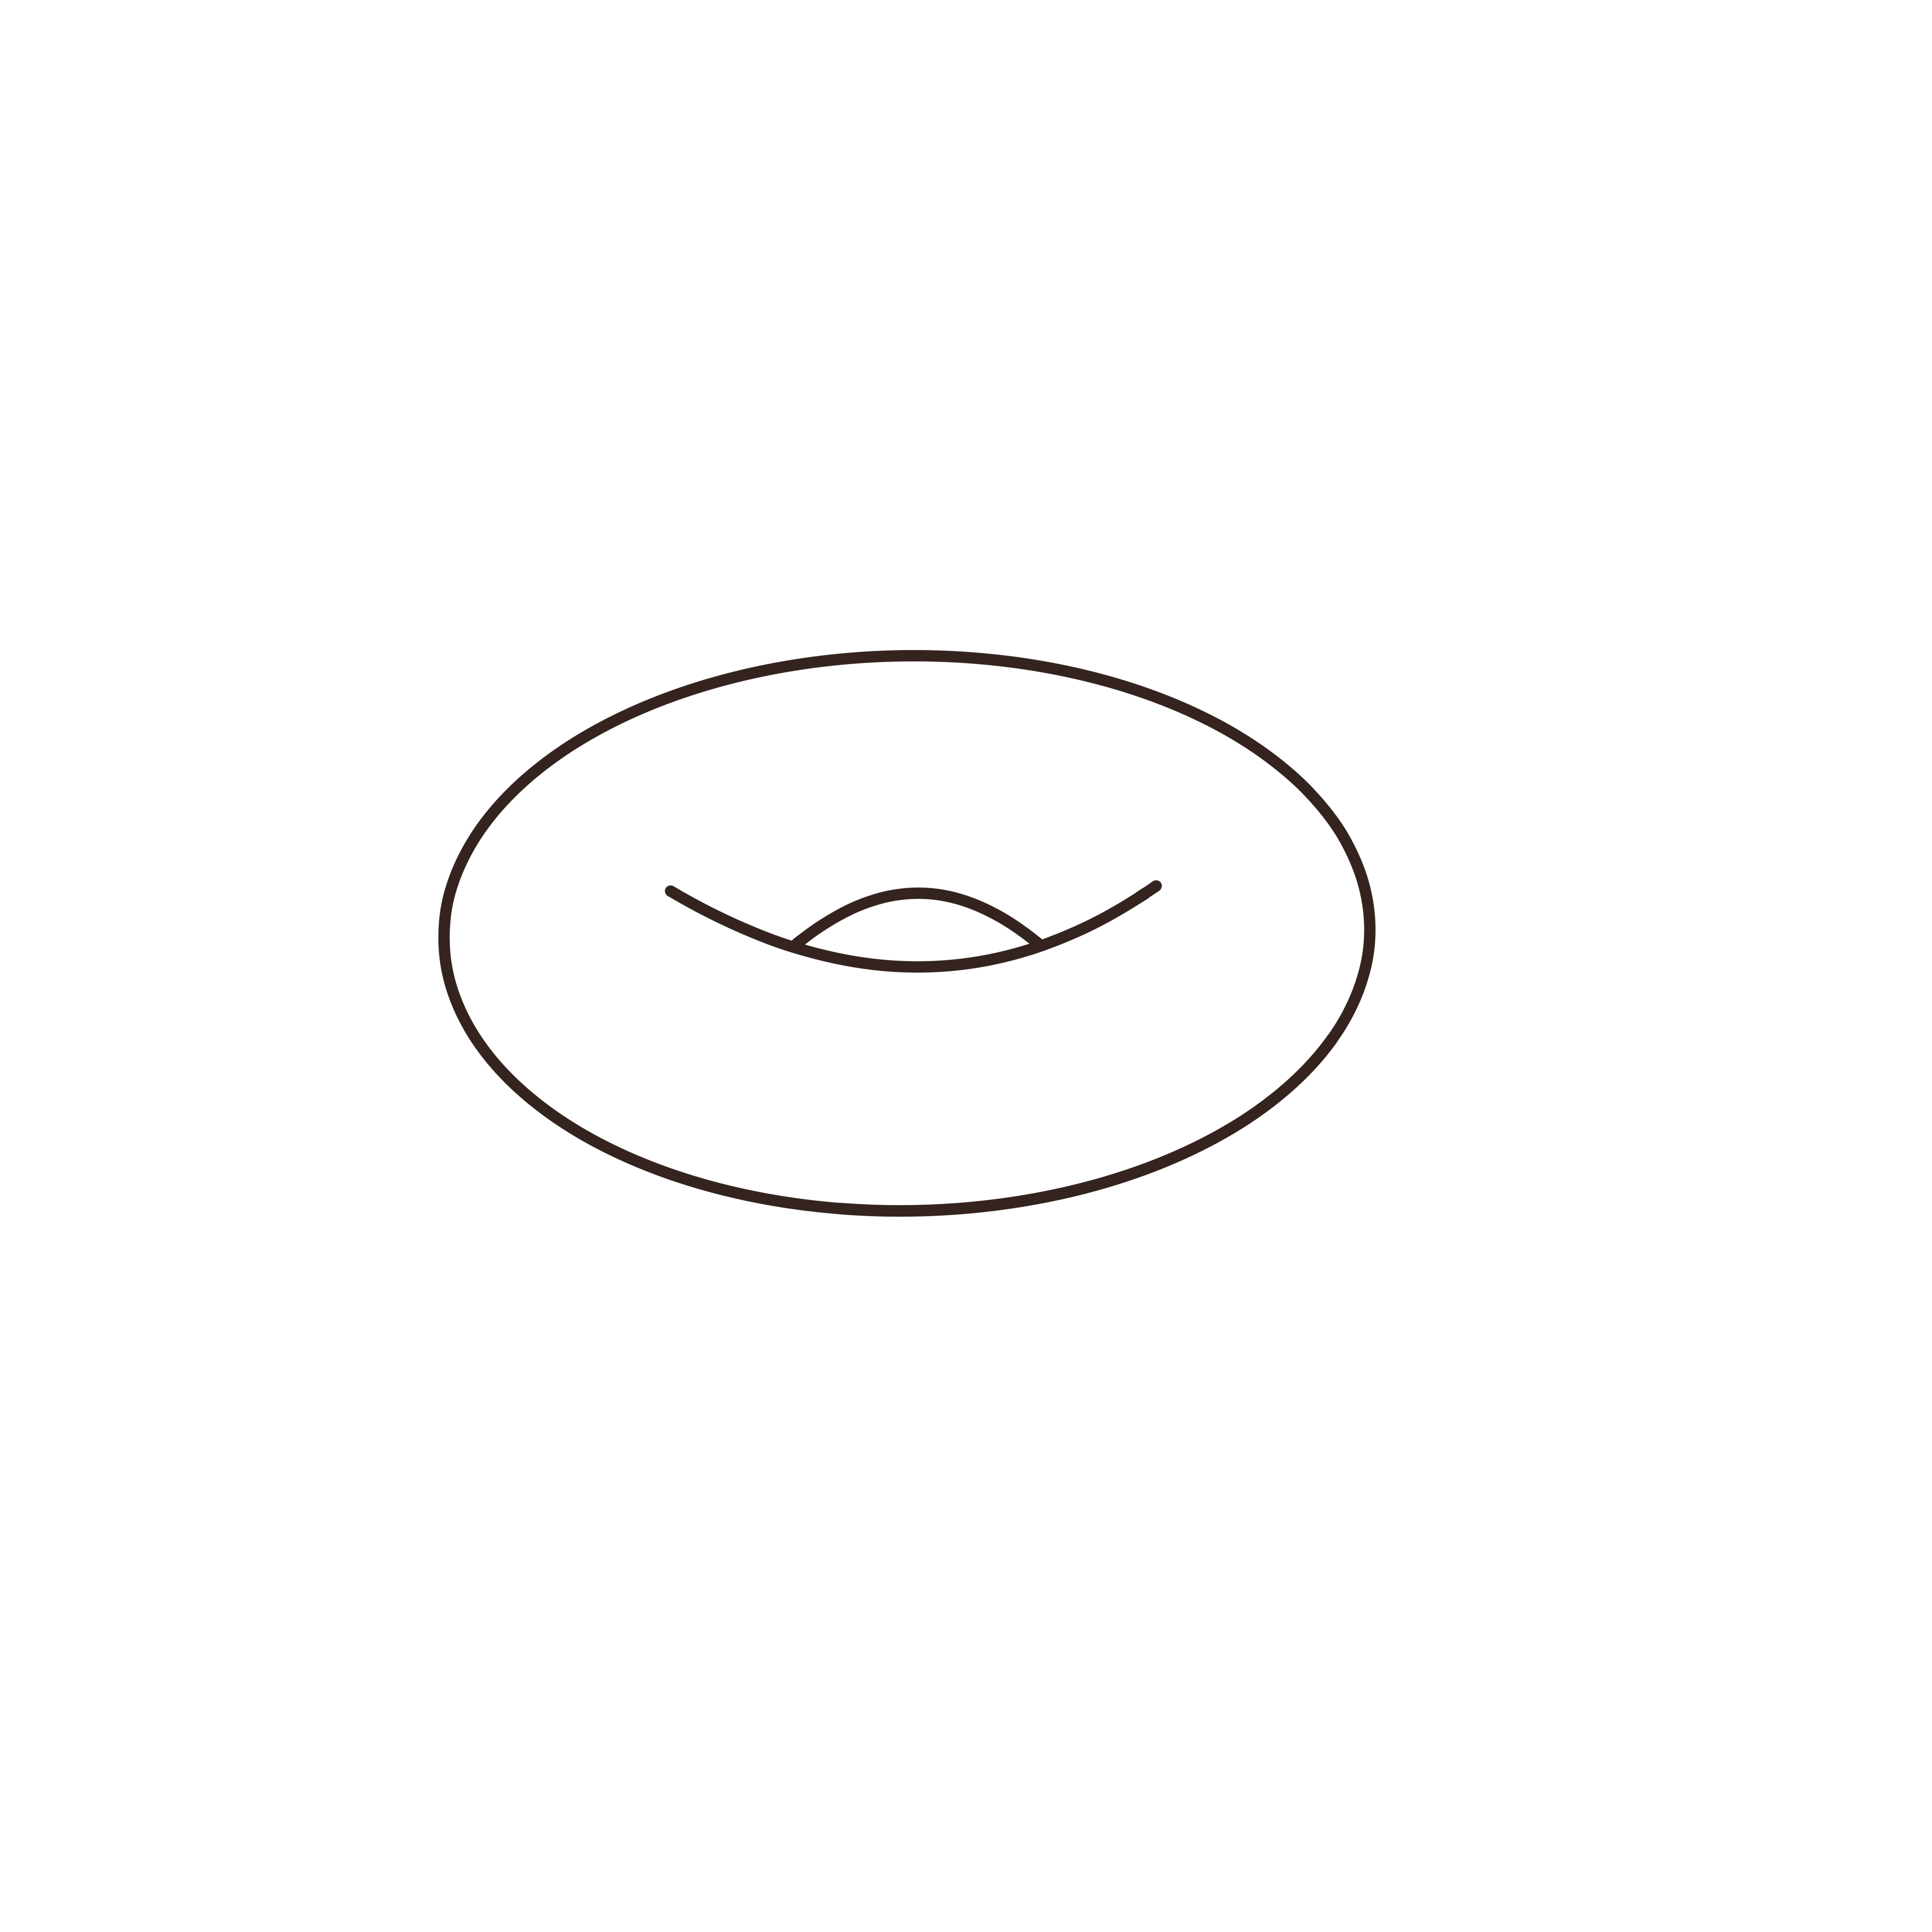
\includegraphics[width=0.3\linewidth]{imagenes/toro.png}
	\caption{Toro}
\end{figure} 

Es un ejercico simple pero extenso  demostrar que  el toro así definido es homeomorfo a la estructura de donut que se suele estudiar.

Por su parte, el \textit{plano proyectivo} parte del mismo conjunto $X$ y se construye con las identificaciones:
\begin{align*}
(x,-1)\equiv(-x,1) \quad x\in [-1,1]\\
(-1,y)\equiv(1,-y) \quad y\in [-1,1] 
\end{align*}
Utilizando en este caso también la topología cociente. Equivalentemente se puede definir como el espacio cociente que resulta de identificar los puntos diametralmente opuestos de $S^2$.


\begin{figure}[h]\label{fig:planoproyectivo}
	\centering
	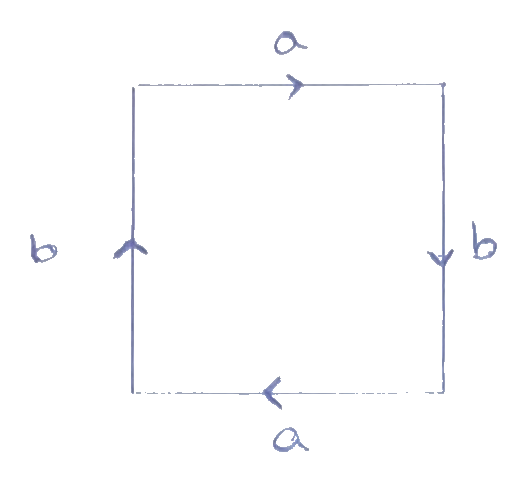
\includegraphics[width=0.3\linewidth]{imagenes/planop.png}
	\caption{Plano proyectivo}
\end{figure} 

Las gráficas [REF IMG1] y [REF IMG2] nos permiten establecer una notación algebraica para referirnos a estas superficies: 
Inciando en una arista cualquiera recorremos la figura en el sentido de las agujas del reloj y anotamos cada letra que encontramos, agregando un exponente a la -1 en caso de que el sentido de su flecha sea inverso al del recorrido. Con esto describiríamos [REG IMG1] como $aba^{-1}b^{-1}$ y [REF IMG2] como $abab$. La notación nos permite referirnos a nuevas superficies fácilmente, por ejemplo, $aba^{-1}b$ se correspondería con [REF IMG4] y $aa^{-1}$ con [REF IMG5]. 


\begin{figure}[h]\label{fig:botelladeklein}
	\centering
	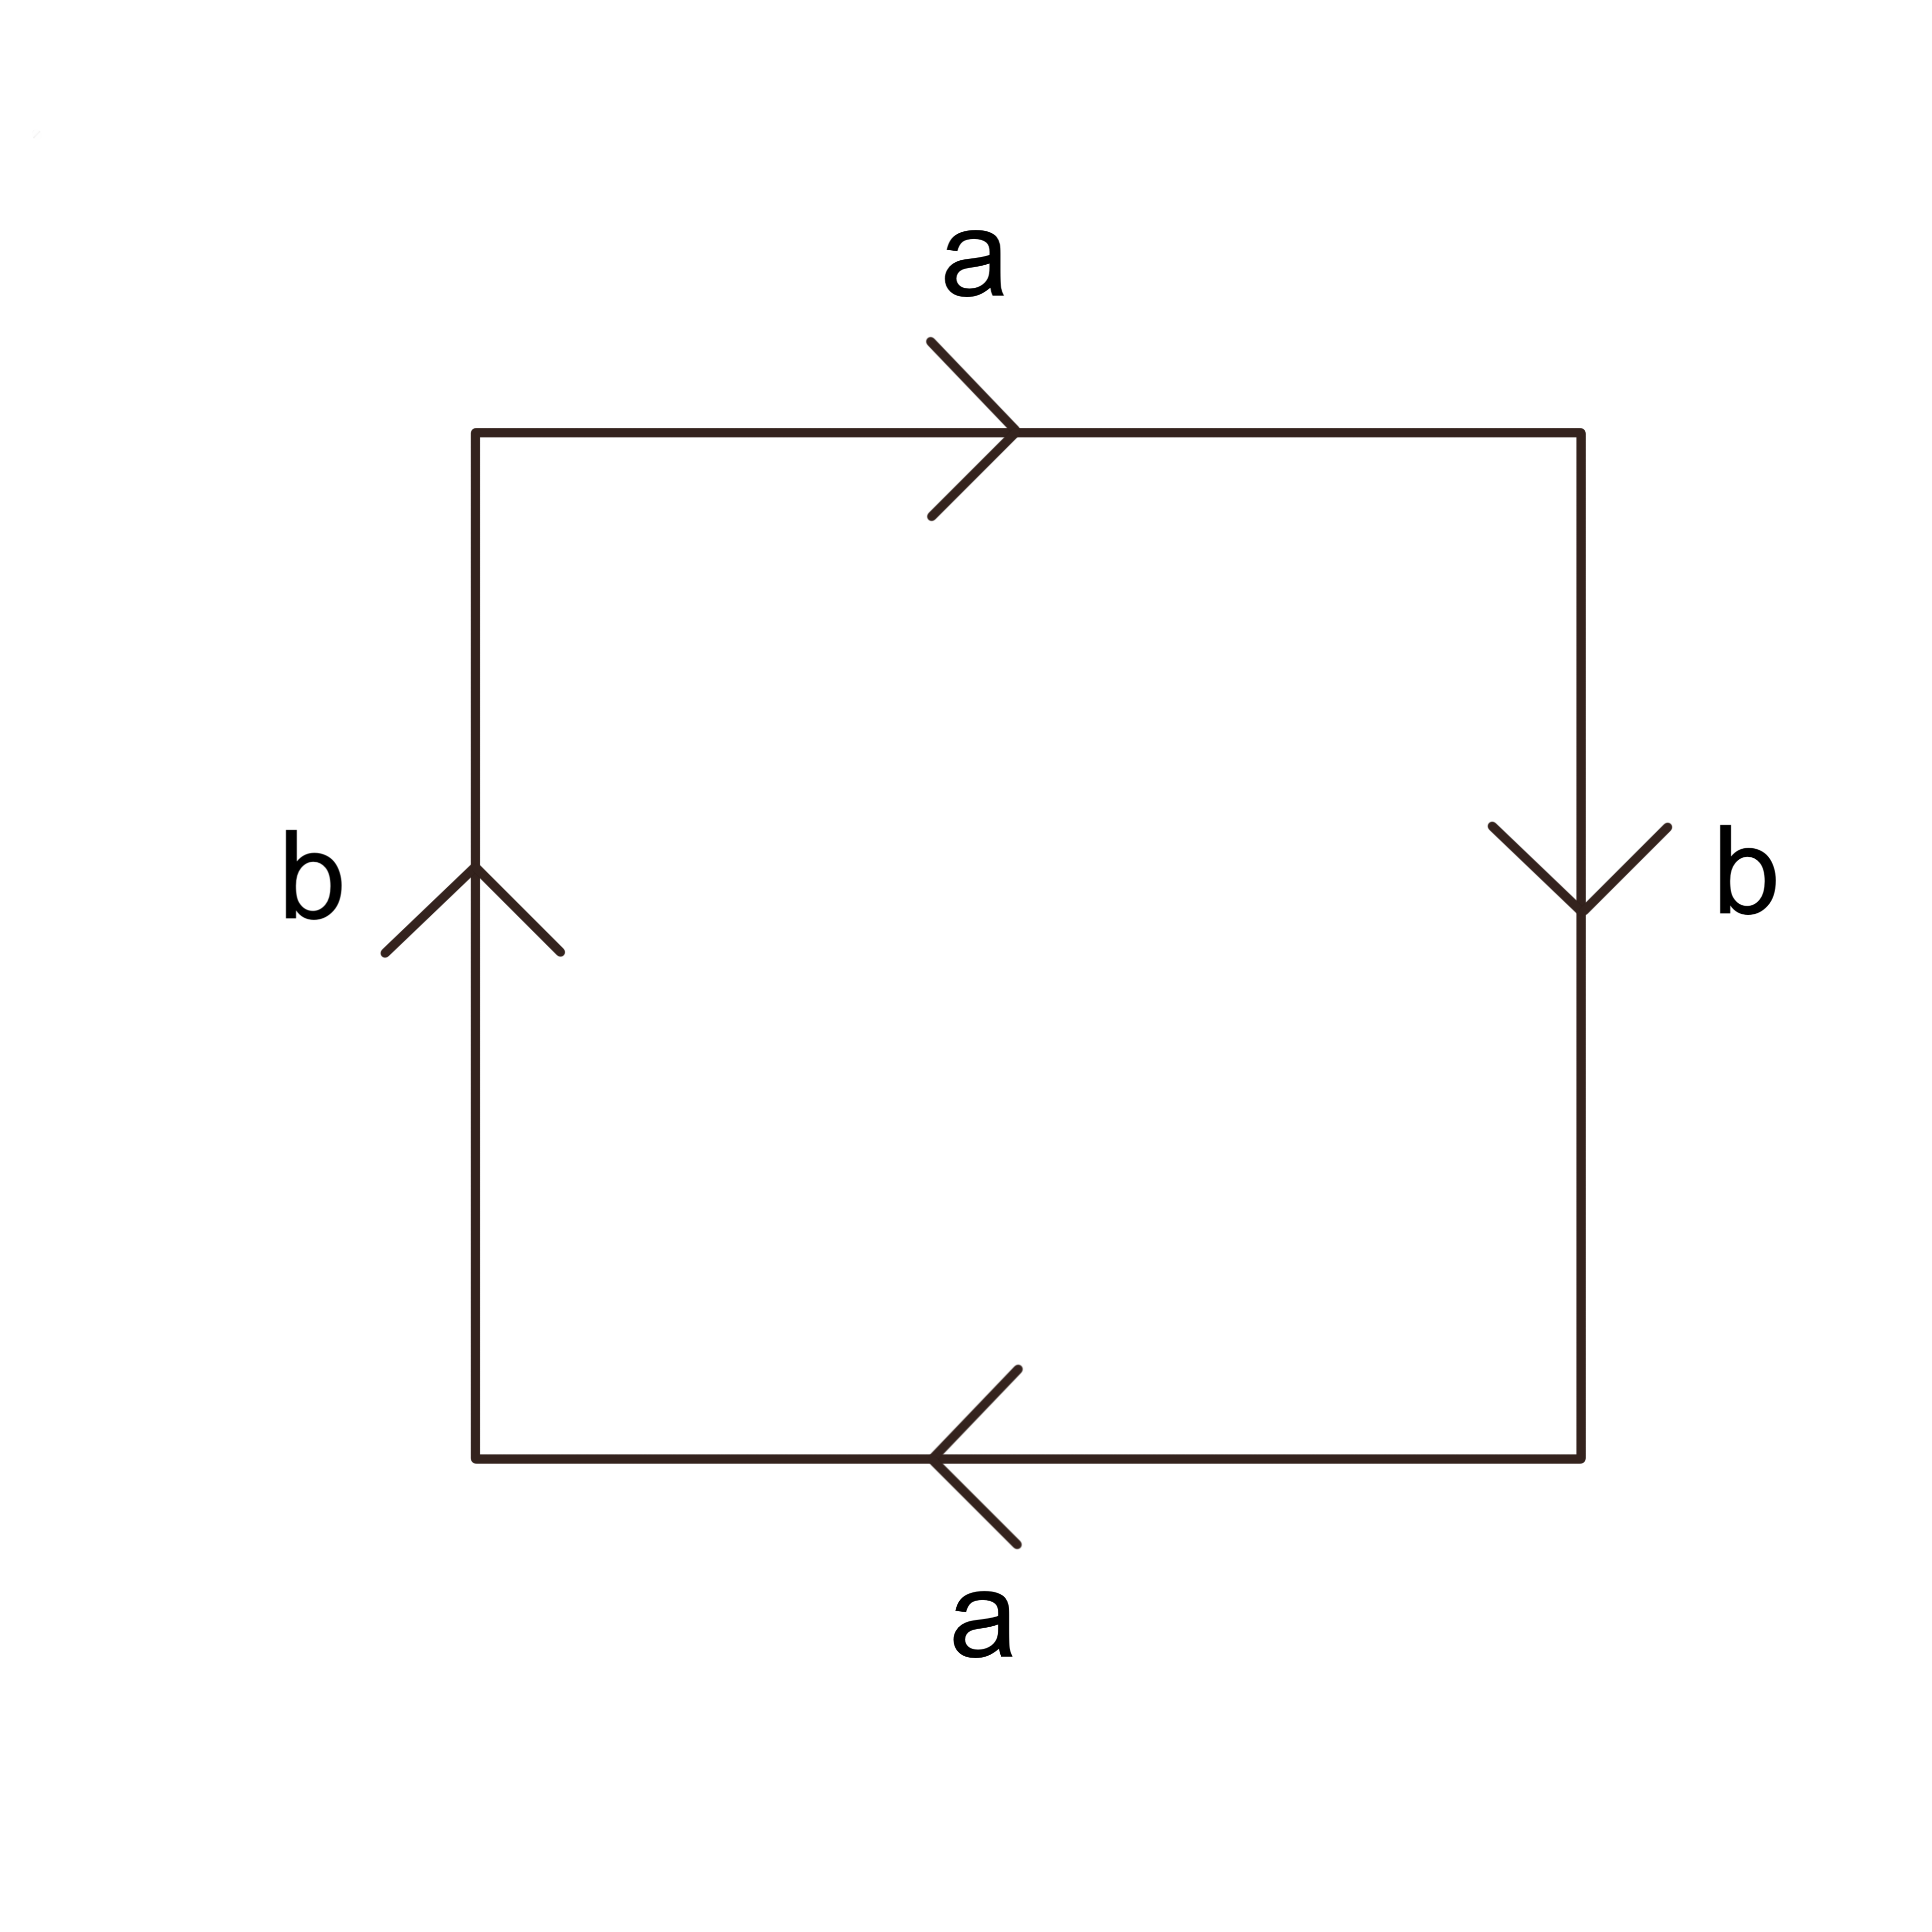
\includegraphics[width=0.3\linewidth]{imagenes/klein.png}
	\caption{Botella de Klein}
\end{figure} 


[IMAGEN 5]

El siguiente lema [REF A LEMA] nos permitirá comprobar que todas las superficies tratadas hasta ahora son compactas.

\begin{lema}
	Sea $X$ un espacio topológico e $Y$  un espacio cociente que resulta de identificar puntos en $X$. Entonces:
	\begin{align*}
	\text{$X$ compacto}\Rightarrow\text{$Y$ compacto}
	\end{align*}
\end{lema}
\begin{proof}
	Sea $f:X\longrightarrow Y$ la función cociente que asocia a cada punto su clase de equivalencia; $f$ es claramente sobreyectiva y, por ser cociente, es continua.\\
	Siendo $X$ compacto tenemos entonces que $f(X)=Y$ también lo es.
\end{proof}



Definimos a continuación un operador que nos permitirá generar infinidad de nuevas superficies partiendo de las ya estudiadas (de hecho, si se me permite el \textit{spoiler}, podremos generar todas las superficies compactas posibles).



\begin{defin}\label{defin:sumaconexa}
	Dadas dos superfices $S_1$ y $S_2$ podemos definir la suma conexa de ambas, $S_1\#S_2$, como la superficie generada a partir de los siguientes pasos:
	
	\begin{enumerate}
		\item 
		Para cada $S_i$ tomamos un subconjunto $D_i\subset S_i$ homeomorfo al disco cerrado de dos dimensiones $E^2$. Llamamos $S'_i$ al complementario del interior de $D_i$.
		\item 
		Sea $\phi_i$ el homeomorfismo que manda $D_i$ al disco cerrado $E^2$, definimos el homeomorfismo $\psi$ que manda la frontera de $D'_1$ a la frontera de $D'_2$ como:
		\begin{align*}
		\psi = ((\phi_{2}\mid_{fr(D_2)})^{-1}) \circ (\phi_1\mid_{fr(D_1)})
		\end{align*}
		\item 
		Definimos entonces $S_1\#S_2$ como $S'_1\cup S'_2$ dotado de la topología cociente que resulta de identificar los puntos $x$ y $\psi(x)$ para todo punto de la frontera de $D_1$.
	\end{enumerate}
	
	Para confirmar la validez de estar definición hay que aclarar varios puntos:
	\begin{enumerate}
		\item 
		Primero, por qué podemos asegurar en el punto 1 de la definición que existe un subconjunto homeomorfo a un disco.
		\begin{proof}
			Tomamos un punto $p\in S_i$ cualquiera. Como $S_i$ es una 2-variedad, entonces existe un homeomorfismos $g$ que manda un entorno, $U$, del punto $p$ al círculo abierto. 
			
			Tomamos $E_{\frac{1}{2}}$ el disco cerrado de radio $\frac{1}{2}$, y $U'= g^{-1}(E_{\frac{1}{2}})$. Tenemos que $g\mid_{U'}$ es un homeomorfismo de un subconjunto de $S_i$ a $E_{\frac{1}{2}}$ que a su vez es homeomorfo al disco cerrado de radio 1. (HACE FALTA?)
		\end{proof} 
		\item 
		Segundo, tenemos que asegurarnos que en el punto 2 las fronteras de $D_1$ y $D_2$ tienen la misma imagen.
		\begin{proof}
			Comencemos por aclarar una sutileza en la definición: Cuando hablamos de $D_i$ homeomorfos a $E^2$, nos referimos a homeomorfos como subconjuntos de las superficies, no como conjuntos independientes dotados de la topología del subconjunto.
			
			Partiendo de eso, basta con probar que dado un homeomorfismo $f: X\longrightarrow Y$, y el conjunto cerrado $B\subset X$, entonces $f(fr(B)))= fr(f(B))$.
			Para esto basta con probar que dado un homeomorfismo $f: U\subset X \longrightarrow V\subset Y$, con $U$ y $V$ cerrados, se cumple que $f(fr(U)) = fr(V)$. Esto se sigue directamente de que $f(\mathring{B})=\mathring{f(B)}$, que a su vez es resultado inmediato de las propiedades de homeomorfismos. (HACE FALTA?)
		\end{proof}
		\item 
		Tercero, habría que comprobar que, en efecto, el objeto obtenido es una superficie. Es decir, comprobar que todo punto tiene un entorno homeomorfo al disco abierto, que el espacio es T2 y que es conexo.
		\begin{proof}
			
			(HACE FALTA?)
		\end{proof}
		\item 
		Y, finalmente, tenemos que comprobar que esta definición es independiente de los conjuntos $D_i$ escogidos e independiente de los homeomorfismos.
		\begin{proof}
			(HACE FALTA?)
		\end{proof}
	\end{enumerate} 
\end{defin}

[Nota: sigo acaso demasiado la estructura que hay en el libro de massey? es esto un plagio? No sabría plantearlo de otra forma, su hilo argumental tiene todo el sentido del mundo]




\chapter{Algunos resultados de topología}
Cosas que empecé a escribir pero que probablemente no haga falta incluir en el TFG. Son definiciones elementales de topo y algunos lemas

\begin{defin}
	Un conjunto $\mathcal{X}$ es no conexo si existen dos  conjuntos cerrados, $\mathcal{X}_1$ y $\mathcal{X}_2$, tal que $\mathcal{X}=\mathcal{X}_1\cup\mathcal{X}_2$ y $\mathcal{X}_1\cap\mathcal{X}_2=\emptyset$.
\end{defin}
\begin{defin}
	Un conjunto $\mathcal{X}$ se dice conexo si no cumple la definición anterior.
\end{defin}


Para considerar gráficamente el toro se asigna a cada arista de un cuadrado unidad una letra y un sentido. Si dos aristas comparten letra, entonces son puntos identificados según el sentido de la flecha. Mostramos en \ref{fig:toro} la representación visual del toro.


Partiendo de la notación gráfica se puede establecer una notación algebraica. Empezando en uno de los vértices recorremos el borde de la figura en el sentido de las agujas del reloj, si el sentido  de la arista corresponde con el del recorrido entonces escribimos la letra, si es contrario entonces escribimos la letra elevado a -1. En el caso del toro tenemos: $aba^{-1}b^{-1}$ 



\begin{defin}\label{defin:planoproyectivo}
	Se llama plano proyectivo al cuadrado unidad, identificando los puntos:
	\begin{itemize}
		\item 
		$(x,1)$ con $(1-x,0)$ para $0\leq x\leq 1$
		\item 
		$(0,y)$ con $(1,1-y)$ para $0\leq y\leq 1$
	\end{itemize}
	La topología que se considera es la cociente, inducida por el cuadrado cerrado con la topología usual.
\end{defin}

En la figura \ref{fig:planoproyectivo} observamos el plano proyectivo en notación visual.

En notación algebraica el plano proyectivo se escribe $abab$.

Sirviéndonos de la notación algebraica podemos definir \textit{la botella de Klein} como $aba^{-1}b$ 




\begin{lema}{El pseudolema más útil de toda la topología}
	
	Al dilatar, comprimir, trasladar y cortar-identificar una figura, el objeto obtenido es homeomorfo al inicial. ¿Por qué?, se pregunta un matemático, porque todas las transformaciones son continuas. (¿Incluir en el TFG en tono seriesisímo?) 
\end{lema}

¿Ejemplillos de suma conexa de toros y planos proyectivos?

\begin{lema}\label{lema:sumadedosplanosproyectivos}
	La suma conexa de dos planos proyectivos es una botella de Klein.
	\begin{proof}
		Un plano proyectivo se puede entender como el disco unidad en el que se identifican los puntos diametralmente opuestos. Utilizando esta definición seleccionamos el subconjunto $D = \left\{(x,y): |y|\geq\frac{1}{2}, |x|\leq\sqrt{1-y^2} \right\}$, homeomorfo al disco cerrado, para realizar la suma conexa de los planos. En la figura  \ref{fig:parte1SumaConexaDePlanosP} eliminamos el conjunto $D$ e indicamos con líneas discontinuas los segmentos a identificar con la otra superficie.
		
		\begin{figure}[h]\label{fig:parte1SumaConexaDePlanosP}
			\centering
			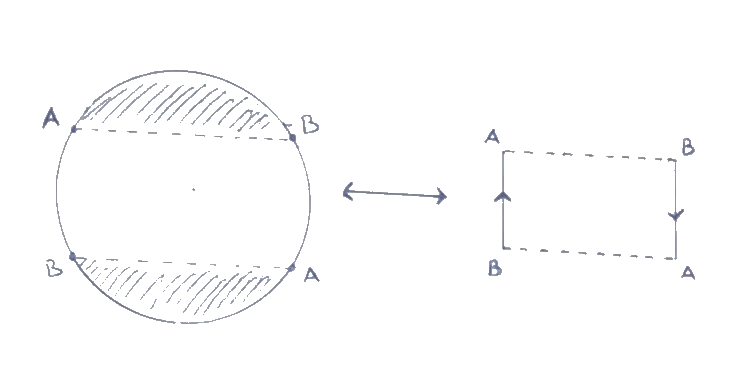
\includegraphics[width=0.7\linewidth]{imagenes/p1planop.png}
			\caption{Plano proyectivo menos un subconjunto homemorfo al disco cerrado}
		\end{figure} 
	
		Tomamos entonces dos planos proyectivos $I$ e $II$ y realizamos la suma conexa:
		
		\begin{figure}[h]\label{fig:sumaconexadepps}
			\centering
			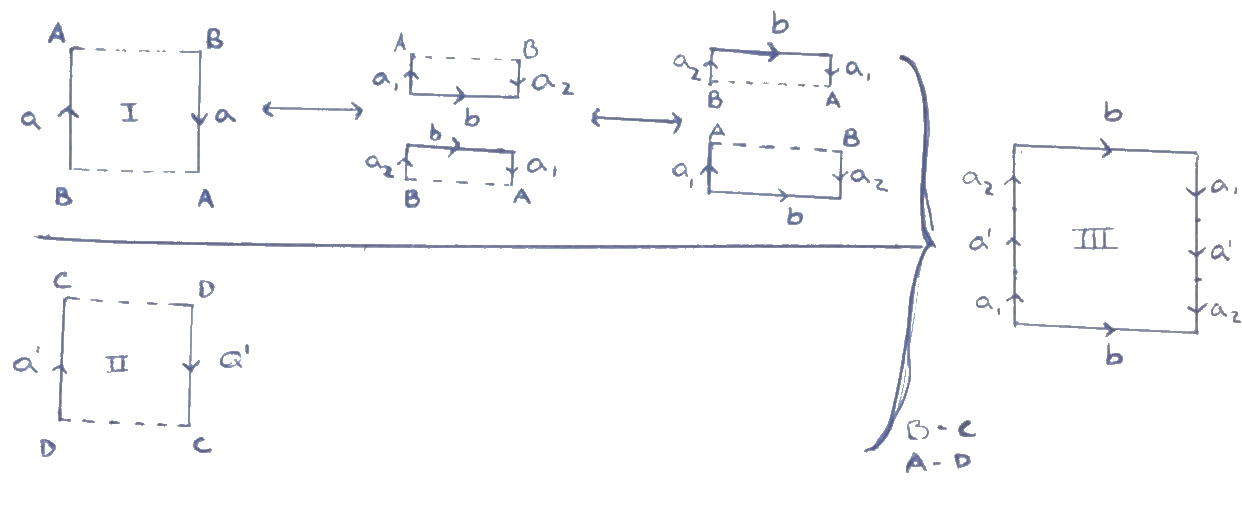
\includegraphics[width=0.8\linewidth]{imagenes/sumapps.png}
			\caption{Suma conexa de planos proyectivos}
		\end{figure} 
		La figura final obtenida ($III$) es una \textit{Botella de Klein}.
	\end{proof}
\end{lema}







\begin{defin}\label{defin:triangulacion}
	Una triangulación de una superficie compacta, $S$, consiste en subconjuntos cerrados, ${T_1, ..., T_n}$, que cubren a $S$ y una familia de homeomorfismos, ${\phi_1, ..., \phi_n}$, que cumplen:
	\begin{align*}
	\phi_i: T'_i \longrightarrow T_i
	\end{align*}
	Donde $T'_i$ es un triángulo del plano $\mathbb{R}^2$. Además, tomando $T_i$ y $T_j$ con $i\neq j$, se cumple una de las siguientes condiciones:
	\begin{itemize}
		\item 
		Son conjuntos totalmente disjuntos.
		\item 
		Comparten un solo vértice en común y solo eso (Llamamos vértice a todo elemento de $S$ que se corresponde por algún $\phi_i$ con un vértice en el plano).
		\item 
		Tienen toda una arista en común y solo eso (Llamamos arista a la imagen de una arista de alguún $T'_i$ por $\phi_i$).
	\end{itemize}
\end{defin}


\begin{teor}{Teorema de Tibor Radó}\label{teor:teoremaDeTriangulacion}
	
	Toda $S$ superficie compacta es triangulable.
\end{teor}(NO LO DEMOSTRAREMOS)




Lemas de triangulación
\begin{lema}\label{lema:lema1detriangulacion}
	Sea $S$ una superficie triangulable entonces una arista lo es de exactamente dos triángulos.
\end{lema}(TODO: FALTA DEMS)

\begin{lema}\label{lema:lema2detriangulacion}
	Sea  $S$ una superficie triangulable y $v\in S$ un vértice en esa triangulación, entonces podemos ordenar el conjunto de todos los triángulos con vértice $v$ cíclicamente,  $T_0, T_1, ..., T_n = T_0$, de manera que $T_i$ y $T_{i+1}$ tienen toda una arista en común para todo $0\leq i\leq n-1$.
\end{lema}(TODO: FALTA DEMS)


\begin{teor}{Teorema de clasificación de superficies compactas}\label{teor:teoremadeclasificacion}
	
	Toda superficie compacta es homeomorfa a una esfera, a una suma conexa de toros o una suma conexa de planos proyectivos.
\end{teor}










\begin{thebibliography}{10}

%% TODO: VER COMO SE TIENEN QUE PONER LAS CITAS
\bibitem{massey} 
    \textsc{William S. Massey}: 
    Introducción a la topología algebraica. 
    \textit{Editorial Reverté} {\bf1} (2006), 1--29.

\bibitem{ian}
    \textsc{Ian Richards}
    \textit{Classification of non compact surfaces...o algo asi}
    
    
\end{thebibliography}
\cleardoublepage


\end{document}
